This chapter follows the implementation process for the project. It is broken up
very similarly to the design section, and details the implementation
difficulties which occurred when implementing each of the components.

\section{Compiler}

The compiler is broken into a pipeline of steps. I implemented these components
in the order that they would be performed by the compiler, and tested them at
each stage (as detailed in chapter \ref{testing}).

I have previously mentioned that the compiler is written in Haskell, and that
choosing a functional language was for the convenience it presents in handling
highly recursive processes such as code generation. However, Haskell presents
another convenience: \gls{lazy-eval}. This allows some of the code to be much
simpler without sacrificing performance.

\subsection{Lexer}

As described in \ref{design-lexer}, the lexer takes the plain source text as
input, and produces a token stream as output. However, for the purpose of
producing reasonable error messages throughout computation, the lexer also has
to track the line number and column at which each token occurs. The
implementation for this functionality is broken up as follows:

\begin{description}
  \item[Reader:] To encapsulate the location tracking behaviour, the
    \texttt{Reader} monad provides a way of reading characters from a string and
    having the line and column values be automatically tracked and updated. Each
    token matcher can then be implemented as something of type \texttt{Reader
    Token}, and can be executed by calling \texttt{run\_reader token\_matcher
    "input string"}. A \texttt{Reader} can fail, in which case it returns
    \texttt{Nothing}. The monad also has the following combinators:
    \begin{itemize}
      \item
        \texttt{(>>=) :: Reader a -> (a -> Reader b) -> Reader b},
        
        which applies the first reader and then (assuming it succeeded) applies
        the second reader, combining the results. This is effectively
        the concatenation of two readers.
      \item
        \texttt{(>>!) :: Reader a -> Reader a -> Reader a},
        
        which applies the first reader and then if it fails, applies the second
        reader instead. This is effectively the union of two readers.
    \end{itemize}
  \item[Token:] Since there are two separate token streams produced during
    compilation, the \texttt{Token} datatype is parameterised by a separate
    datatype, \texttt{RawType}. The \texttt{Token} type tracks the location and
    comes with a small collection of utility functions for token matching which
    are used in the parsing phase, whilst the \texttt{RawType} datatype
    expresses the selection of token types which was described in
    \ref{design-lexer}.
  \item[Lexer:] The lexer then consists of a collection of definitions for
    various instances of \texttt{Reader (Token RawType)}, which are combined
    together to produce a single reader for whatever token is at the head of the
    input source. Repeated application of this reader gives the first token
    stream.
\end{description}

\subsection{Indentation Parser}

Section \ref{design-indent} outlines the procedure by which indentation parsing
is achieved. The token stream produced by the lexer is broken into lines before
having the whitespace stripped out and replaced with \texttt{INDENT} and
\texttt{DEDENT} tokens where necessary. The conversion is performed with a
single pass over the list of lines. The indentation level of the program is
tracked, and when the indentation changes, \texttt{INDENT} or \texttt{DEDENT}
tokens are produced.

The main source of complexity with this implementation is with handling
continuation lines: some lines may be prematurely broken in order to improve
readability. For instance, the statement
\lstinputlisting[firstline=2, lastline=2, language=occam]
    {code/line_continuation.occ}
could be rewritten as
\lstinputlisting[firstline=5, lastline=6, language=occam]
    {code/line_continuation.occ}
to improve readability. In this case, the indentation of the second line must
not be converted into \texttt{INDENT} tokens, and any subsequent lines should
not produce \texttt{DEDENT} lines because of it.

The solution to this is to have a classifier function which determines whether
or not a line has ended with a continuation token\footnote{This is a
well-defined subset of the possible tokens upon which it is acceptable to
prematurely break the line.}. When processing the indentation of a line which
follows one ending with a continuation token, no indentation tokens are
generated and the record of the current indentation level is left unaltered.

\subsection{Parser}

Section \ref{design-parser} explains that the parser for this project is
implemented from scratch, and that it is broken into two parts: the parsing
library, and the Occam parser.

\subsubsection{The Parsing Library}

The parsing library defines a \texttt{Parser} monad along with a collection of
combinators for building parsers. The \texttt{Parser} type is defined
as\footnote{This uses the Generalised Algebraic Data-Types extension to GHC to
allow for more complicated type definitions.}:
\lstinputlisting[language=haskell]{code/parser_monad.hs}
These parser types can be summarised as follows:
\begin{description}
  \item[\texttt{Epsilon}] matches the empty-string.
  \item[\texttt{Match "foo" f}] matches tokens which satisfy the predicate
    \texttt{f}, and displays \texttt{foo} in error messages which concern this
    location in the parse tree.
  \item[\texttt{Union ps}] matches any of the parsers in \texttt{ps}.
  \item[\texttt{Concat p q}] matches the concatenation of parsers \texttt{p} and
    \texttt{q}.
  \item[\texttt{Star p}] matches zero or more repetitions of parser \texttt{p}.
  \item[\texttt{Reduce f p}] matches parser \texttt{p}, but then applies
    \texttt{f} to the result. This is what allows the parse tree to be
    transformed into the \gls{ast}.
\end{description}
Combinations of these parsers can be used to parse any of the grammars that we
will need to parse. A parser can be invoked with:
\lstinputlisting[firstline=10, lastline=11, language=haskell]
    {code/run_parser.hs}
That is, \texttt{run\_parser p ts} will run the parser \texttt{p} on the token
list \texttt{ts}, and produce a list of \texttt{Result}s, each of which is
either \texttt{Success (partial\_parse, remaining\_tokens)} or
\texttt{Failure location description}. The implementation of this function for
each of the parser types is given in appendix \ref{parser-lib}.

By producing all parse trees rather than just one, the parser does not have to
backtrack when a failure occurs\footnote{Arguably the parser is still
backtracking: the lazy evaluation semantics mean that the parse trees are
computed in exactly the same order as a backtracking parser, but the code is
simpler.}, and it is easy to debug ambiguous grammars as the different parses
will both appear in the results list. Additionally, when no \texttt{Success}
instances appear in the results list, the parse has failed and the
\texttt{Failure} instances give a selection of potential failure locations to
consider for error messages. The heuristic that I have used is to display the
\texttt{Failure} which has the location furthest into the source text. This has
proven to be reasonably accurate in the simple syntax error cases that I have
considered.

When a parser combinator fails, it will produce a \texttt{Failure} rather than a
success. Naturally, almost every branch of a \texttt{Union} will be a
\texttt{Failure}, so this can lead to there being a large number of
\texttt{Failure} instances, often identical to several other instances in the
results list. This was a significant performance issue, but was easily solved by
removing duplicate entries from the results list generated at each level of the
execution of the parser\footnote{The example program that I was testing my
parser on would parse in 3 seconds prior to the change, and 0.07s afterwards.}.

To facilitate writing parser rules, the parser library also includes the
following infix combinators:
\begin{description}
  \item[\texttt{(|||) :: Parser a -> Parser a -> Parser a}],

    An infix representation of \texttt{Union} between two parsers.

    \texttt{p ||| q = Union [p, q]}.
  \item[\texttt{(+++) :: Parser a -> Parser b -> Parser (a, b)}],

    An infix representation of \texttt{Concat}.

    \texttt{p +++ q = Concat p q}.
  \item[\texttt{(>>>) :: Parser a -> (a -> b) -> Parser b}],

    An infix representation of \texttt{Reduce}.

    \texttt{p >>> f = Reduce f p}.
\end{description}
Together, these combinators allow a parser definition such as
\lstinputlisting[firstline=3, lastline=6, language=haskell]
    {code/infix_parser.hs}
to be rewritten as
\lstinputlisting[firstline=10, lastline=13, language=haskell]
    {code/infix_parser.hs}
It is arguably more clear what is being parsed by the second version than the
first. Note the type \texttt{L a}, which denotes an \texttt{a} which is
additionally tagged with a source location.

The one remaining quirk of the parsing library is that due to the way that the
combinators are implemented, it is necessary to explicitly denote left-recursive
grammars so that they can be treated differently:
\lstinputlisting[language=haskell]{code/left_recursion.hs}

\subsubsection{The Occam Parser} \label{occam-parser-impl}

Implementing the Occam parser was mostly a case of transcribing the Occam
grammar as described in \cite{jones}. However, directly transcribing the rules
for expressions gave the following definition:
\lstinputlisting[firstline=2, lastline=14, language=haskell]{code/expression.hs}
Parts have been excluded for the sake of brevity. A large number of the rules
here start with the same component: \texttt{operand}. This meant that when the
expression being parsed was, for example, \texttt{(complicated expression) * 2},
the \texttt{complicated expression} would be parsed from scratch for every
branch of the union up until the branch for multiplication expressions. By
refactoring this code into the following, the parsing time was reduced by 97\%:
\lstinputlisting[firstline=17, lastline=31, language=haskell]
    {code/expression.hs}

One major divergence from the grammar rules in the source materials was to parse
the left hand side of assignments, the right hand side of inputs, and all
channels as expressions. The set of valid syntactic forms that can be in these
positions is a strict subset of the set of expressions, but parsing in this
manner allows the compiler to produce more meaningful error messages when the
user has mixed up types.

\subsection{Semantic Analysis}

Similar to the parser, the semantic analysis phase is broken into two parts: one
part provides the basic building blocks for the semantic analyser, and the other
provides the specific analysis for Occam.

\subsubsection{The SemanticAnalyser Monad}

Semantic analysis is the stage which is responsible for most of the feedback
which is sent to the user. Thus, it has to be capable of producing error
messages or warnings whilst simultaneously transforming the abstract syntax and
aggregating various global information such as static data. The
\texttt{SemanticAnalyser} monad encapsulates this functionality:
\lstinputlisting[language=haskell]{code/semantic_analyser.hs}
The \texttt{Environment} datatype contains all variables that are currently in
scope. For each variable, its type and the location of its declaration are
stored. The type information is used for performing type checks throughout the
remainder of the analysis, whilst the location is used purely for generating
useful error messages.

When code has to refer to variables which are syntactically in scope but are at
an unknown location relative to the workspace of the code, they must be accessed
via the \textit{\gls{static-chain}}. The \texttt{StaticChain} datatype describes
stores the current state of the static chain, and is used to identify the static
level and offset of variables.

The \texttt{State} datatype tracks properties about the program that need to be
accumulated before code generation can take place. The number of errors produced
will determine whether or not compilation continues after the semantic analysis
finishes\footnote{Trivially, if the number is non-zero then compilation halts.},
and the values \texttt{next\_static\_address} and \texttt{static} aggregate all
of the static constants that are defined throughout the program.  As described
in \ref{static-blob}, these need to be treated separately from the program code.

Finally, the \texttt{SemanticAnalyser} monad is an encapsulation of the full
semantic analysis process, allowing the \texttt{AST} to be transformed into an
\texttt{AnnotatedAST} whilst checking that the program makes sense. The usage
pattern for the monad is:
\lstinputlisting[language=haskell]{code/semantics.hs}
This would be the function for checking an \texttt{AST} node called
\texttt{Foo}. The semantic analysis would be performed, and some number of
warnings may be produced. If the code is invalid, some errors may be produced.
When such an error occurs, the analyser may try to guess an alteration which
would fix the code (purely so analysis can continue and further errors can be
found). If no errors occurred, or the errors were not fatal, then the analyser
would return an \texttt{AnnotatedAST.Foo}, and update the state in the
\texttt{SemanticAnalyser} accordingly.

\subsubsection{The Occam Semantic Analyser}

The semantic analysis for the compiler consists of a collection of functions of
the form described above. The functions perform tasks such as verifying that all
referenced variables have been declared and are in scope. The analyser also
produces warnings when variables are declared with the same name as other
variables in scope. Where expressions are required to be compile-time constants,
the analyser verifies this and computes the value of the constants. Since all
channels and \gls{l-value}s have been parsed as expressions, the type of these
expressions must be checked to verify that it makes sense to assign to them, or
to treat them like channels.

Below is listed a program which contains mistakes which are detected by the
analyser and result in errors and warnings. The compiler realises that this
program does not make any sense and refuses to produce code for it:
\lstinputlisting[language=occam]{code/error.occ}
Executing the compiler on this program results in the following output:
\lstinputlisting[breaklines=true]{code/error_example.txt}

\subsection{Code Generation}

The code generation stage is the largest part of the compiler. There are several
reasons why this is the case:

\begin{itemize}
  \item
    As mentioned in \ref{code-gen}, it is necessary to compute unique labels
    throughout the code generation process. However, to make these more
    readable, each label consists of a name which corresponds to its purpose,
    and a unique integer which disambiguates the labels.
  \item
    When compiling expressions, the compiler may make use of the register stack
    in the transputer to store intermediate values. However, these are not
    guaranteed to be conserved if the process is descheduled, so it is necessary
    to avoid using instructions that can cause the process to be descheduled
    whilst computing the value of expressions.
  \item
    When compiling a particularly complicated expression, the number of
    registers required to store all intermediate values may exceed the register
    stack. Sometimes this can be resolved by reordering the computation of the
    components of the expression, but often it is necessary to allocate
    temporary variables to store the intermediate values.
  \item
    When compiling \texttt{PAR} constructs, it is necessary to know how much
    stack space is going to be required by each of the sub-processes before the
    code for the construct can be generated. However, generating the code for
    the sub-processes requires information about where the process is located in
    memory so that references to external variables can be resolved.
    
    To solve this seemingly circular dependency, the code generation is broken
    into two phases. During the first phase, the amount of space required by
    each component of the program is computed, and then during the second phase
    this information is used to generate the code. The first phase could have
    easily been performed as part of the semantic analysis, but the advantage of
    having it here is that the code for generating a component is in exactly the
    same place as the promise about how much space that component will take.
  \item
    In order to facilitate debugging, the compiler generates comments that
    describe what each part of the assembly code is doing. These comments
    include fragments of the original source code so that the assembly can
    easily be cross-referenced with the Occam code that generated it.
\end{itemize}

Figure \ref{code-example} shows a complete example of the code generated by
compiling a short example program. The metadata file contains information needed
to execute the program which can't be expressed in the program code. This
includes the static data\footnote{This could technically be encoded as a vast
sequence of \texttt{ldc} and \texttt{stnl} instructions, but it would be
incredibly inefficient.} and the amount of memory required to run the program.
Note that while the code only allocates four words (16 bytes) of space, it
implicitly uses a small number of additional words as part of the implementation
of task switching and alternative input, as the Transputer did. This accounts
for the additional six words (24 bytes) which is reported in the
\texttt{root\_process\_size} field of the metadata file.

\begin{figure}[p]
  Input program:
  \lstinputlisting[language=occam]{code/if.occ}
  Generated metadata file:
  \lstinputlisting[language=json]{code/if.json}
  Generated assembly file:
  \lstinputlisting[language=assembly]{code/if.s}
  \caption{Files generated by compiling a small program.}
  \label{code-example}
\end{figure}

\section{Assembler} \label{assembler}

The assembler consists mostly of two monolithic enumerations containing all of
the operations in the program and their corresponding encoded values. In order
to make these easier to maintain, I created an enumeration file format and
a tool which compiles that file to C++ code for parsing and stringifying the
enumeration values. Figure \ref{direct-enum} shows the enumeration file for the
direct instructions, and figure \ref{direct-h} shows the header file that is
generated. Omitted is the generated source file which implements the
\texttt{toString} and \texttt{fromString} functions. There is a similar
enumeration file for the indirect instructions.

\begin{figure}[H]
  \lstinputlisting[language=enum]{code/Direct.enum}
  \caption{The \texttt{.enum} file for direct instructions.}
  \label{direct-enum}
\end{figure}
\begin{figure}[H]
  \lstinputlisting[language=c++]{code/Direct.h}
  \caption{The \texttt{.h} file generated from the \texttt{.enum} file.}
  \label{direct-h}
\end{figure}

\subsection{Parser}

The syntax for the assembly language is briefly described in \ref{asm-syntax}.
However, more explitly, the syntax can be parsed by this regular
expression\footnote{If you are unfamiliar with C++11 raw string literals, the
basic syntax is \texttt{R"foo(Some string)foo"}, which denotes the string
\texttt{"Some string"}, but will not expand any escape sequences and may contain
any characters except for the sequence \texttt{)foo"}. Typically, the identifier
\texttt{foo} can be omitted, which leaves \texttt{R"(Some string)"}.}:
\lstinputlisting[language=c++]{code/asm_regex.cc}

The numbers (and the letter A) in the comments correspond to the group which is
matched by its contents. These groups can then be used to disect the line after
it has matched.  The assembler performs basic checks that the line makes sense
before converting it into an internal representation of an instruction.

\subsection{Bytecode Generation}

Once the instructions are parsed, they have to be encoded in the variable-length
instruction format of the Transputer bytecode. The implementation is more or
less exactly as described in \ref{var-len}: the instructions are generated under
the assumption that all the offsets for labels are correct, and then regenerated
if those offsets change. In practice, this seems to converge in no more than
5-10 iterations, but I have not attempted to prove any bound on the number of
iterations. Once the bytecode has converged, it is written to the bytecode file.

\subsection{Disassembly}

In order to facilitate debugging, I also implemented a disassembler which can
display the contents of a bytecode file in a human readable format. This only
required approximately 100 additional lines of code, and allows the variable
length encoding to be examined:

\begin{minipage}{.3\textwidth}
  \lstinputlisting[language=assembly]{code/tiny.s}
\end{minipage}
\begin{minipage}{.6\textwidth}
  \lstinputlisting{code/tiny.diss}
\end{minipage}

\section{Runtime System}

The runtime system consists of three separate binaries, one for each of the
components described below. There is a large amount of code shared between them,
and a similarly large amount of code which is not specific to this
project\footnote{All of the code used in this project was written by me, but
some of it is utility code that I have written in the past.}.

\subsection{Virtual Machine}

The virtual machine has 58 instructions in total, of which 16 are the standard
direct instructions listed in \ref{assembler}. Of these, five are debugging
instructions that allow the program to print information to the console of the
machine which is running the code. The virtual machine executes a byte at
a time, and throws exceptions if the instructions are unrecognised or invalid.
It also performs bound checking for both the instruction pointer and any memory
access to ensure that misbehaviour by the program is caught and dealt with
appropriately. However, the bound checking can be disabled at compile time to
speed up execution by about 20\%. The implementation for each of these
instructions is built into the \texttt{VM} class.

The \texttt{vm} binary is a thin wrapper around the \texttt{VM} class, and
allows a simple (non-distributed) program to be executed locally. The usage is
as follows:
\lstinputlisting{code/vm.help}

Without compiler optimisations, the virtual machine runs at approximately 27MHz.
With compiler optimisations, that increases to 150MHz. By disabling bound checks
and features which are only required for the distributed environment, that can
be increased to 240MHz\footnote{Performance figures generated by running
programs on a 4GHz i7.}.

\subsection{The Distributed Version}

The layout of the distributed system is best described by Figure
\ref{dist-model}. Green boxes are part of the \texttt{master} binary, and
blue boxes are part of the \texttt{worker} binary.

\begin{figure}[H]
  \centering
  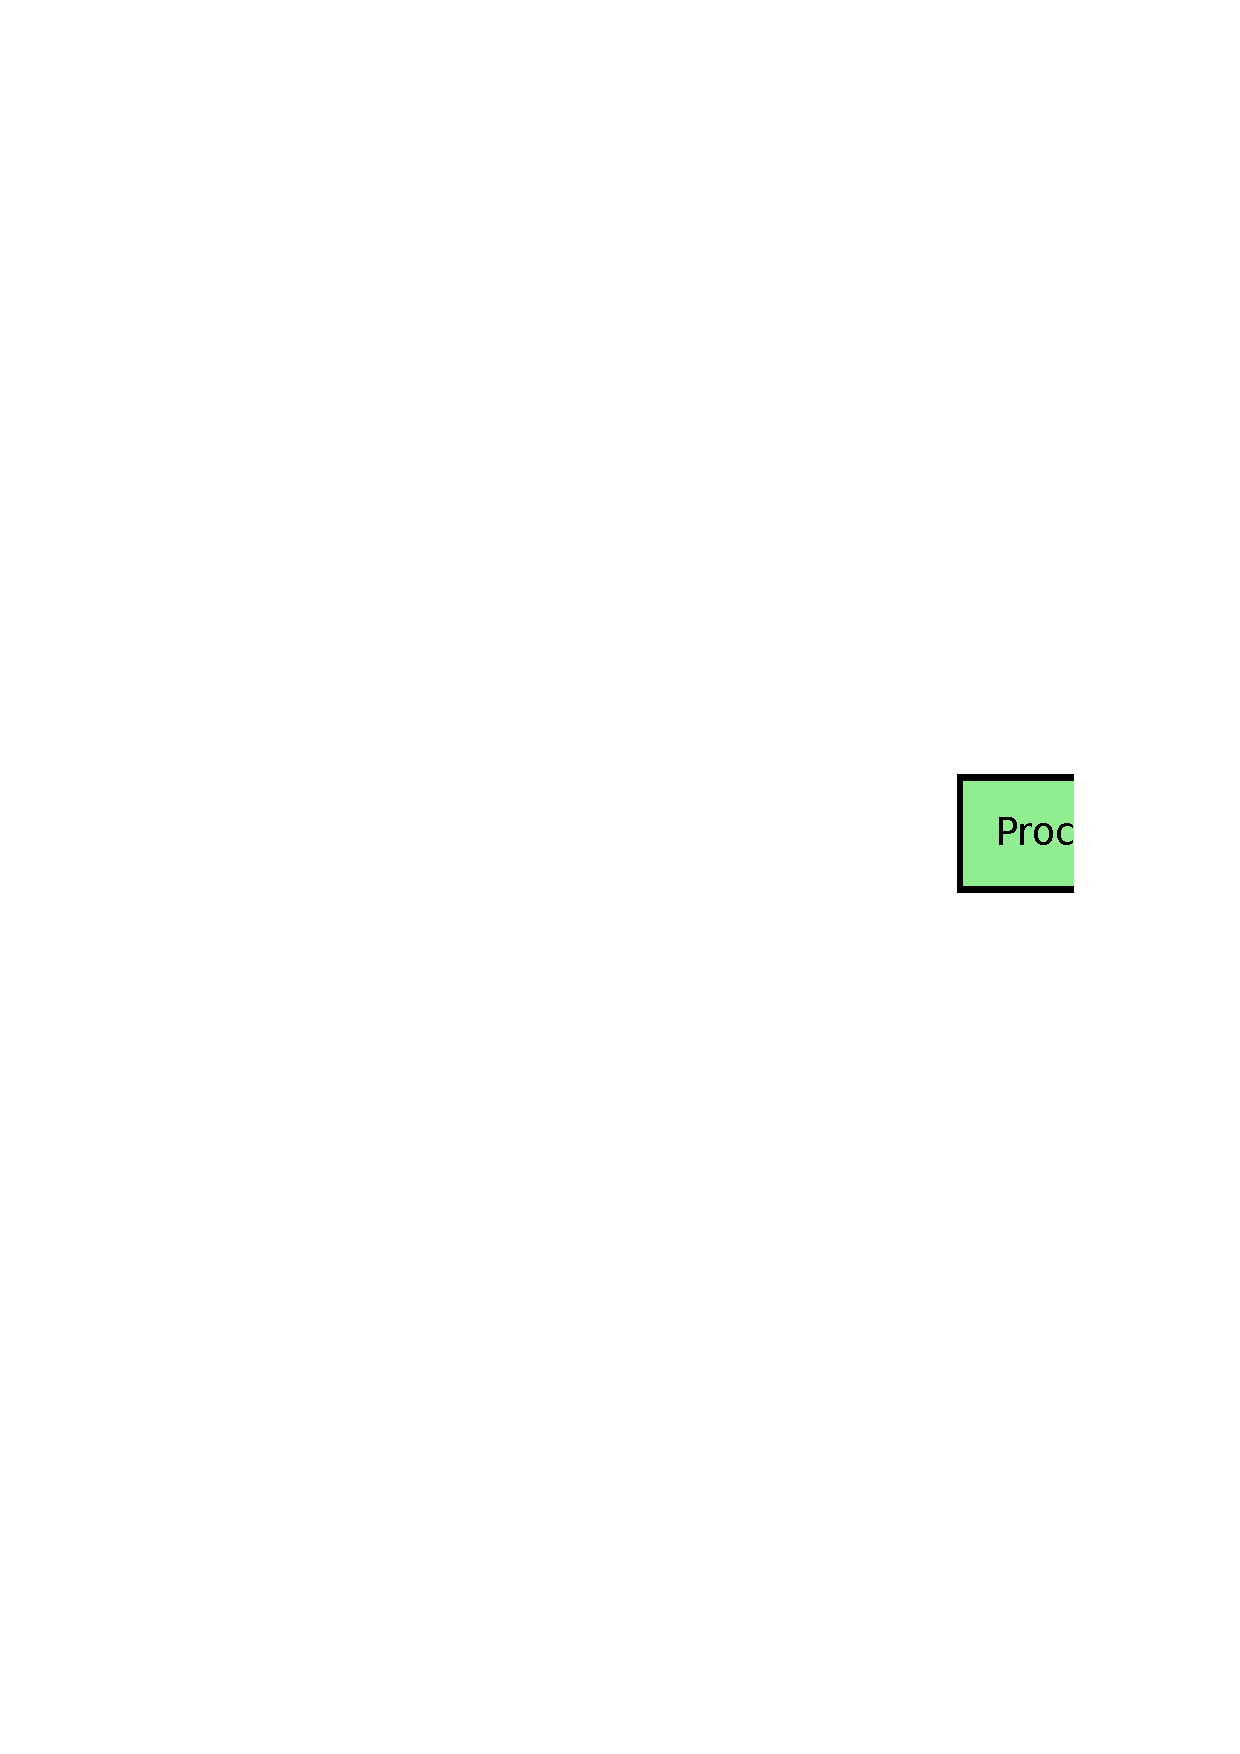
\includegraphics[width=0.4\textwidth]{diagrams/distributed_system}
  \caption{The layout of the distributed runtime system.}
  \label{dist-model}
\end{figure}

\subsection{ProcessTree}

The process heirarchy is tracked via the \texttt{ProcessTree} class. This class
represents the process tree, and provides methods which correspond to each of
the key events (process creation, process termination, ancestry queries). If
a process exits before its children, the process tree will detect this and throw
an error.

\subsection{ProcessMaster}

As described in \ref{process-master}, the \texttt{ProcessMaster} class is
responsible for initializing the \texttt{ProcessServer} on each of the workers.
It is then responsible for serving requests for new instances, and for updating
the process tree when instances start or end. However, channel communication
between the process servers is handled by the \texttt{ChannelMaster} class.

\subsection{ChannelMaster}

The \texttt{ChannelMaster} class handles inter-machine channel communication.
This is achieved through a simple protocol which encodes channel events and
transmits them over the network. The protocol tries to perform as much work as
possible on the process servers, and only sends events to the process master
when it is necessary. The events for a given channel are used to maintain
a small state machine which represents that channel. Figure \ref{channel-master}
shows the state transition diagram for a single channel.  The edges are labelled
with the name of the event which causes the transition, but the messages which
are sent as a result of the transitions are omitted.

\begin{figure}[h]
  \centering
  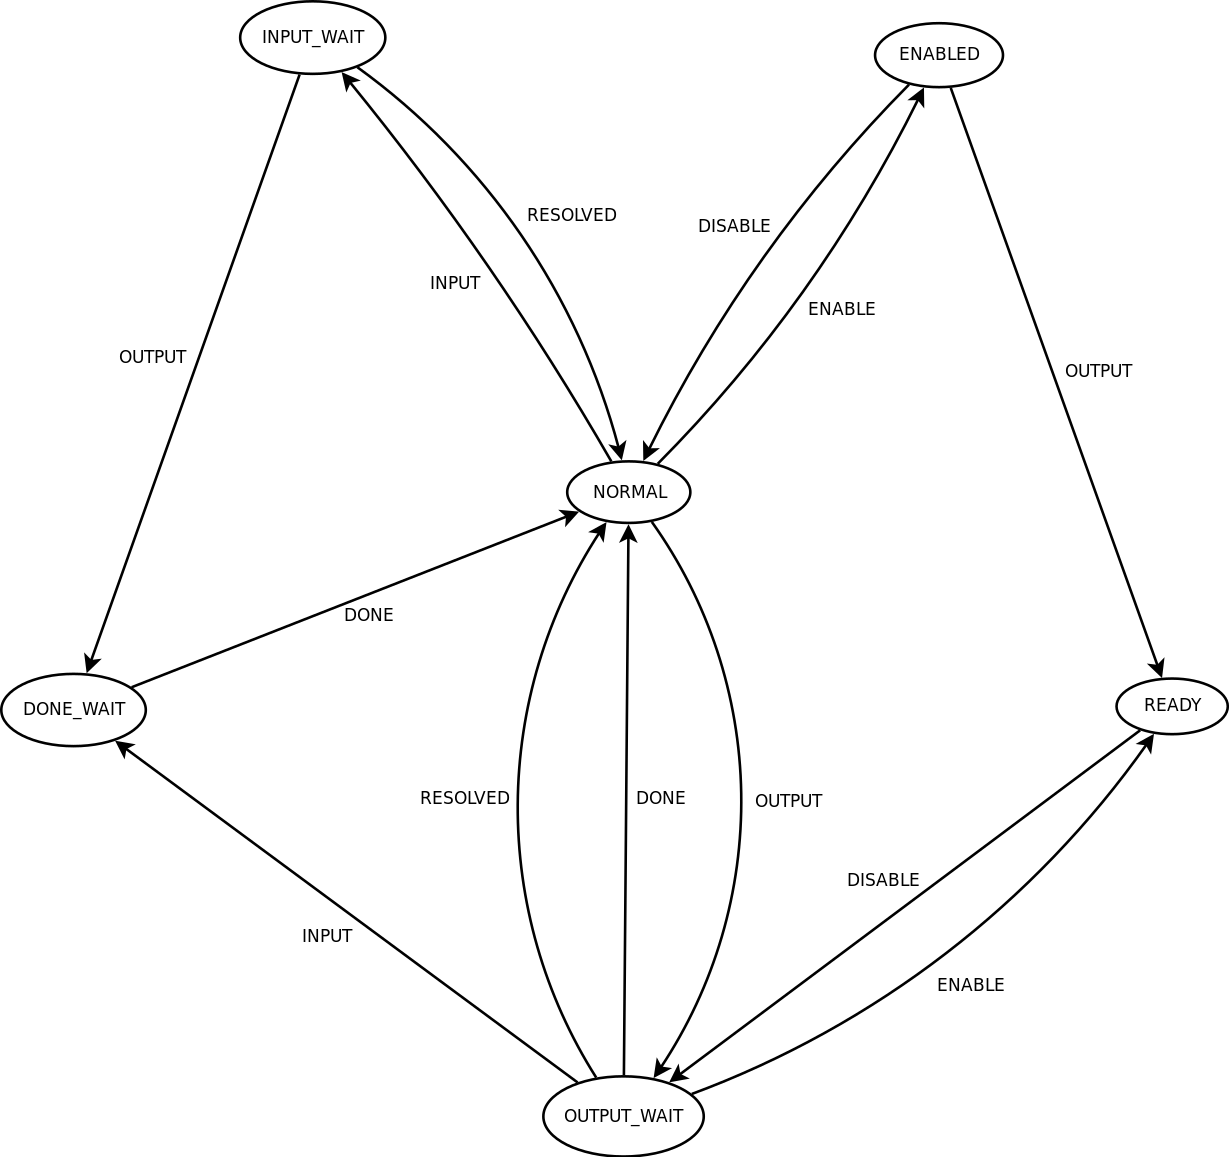
\includegraphics[width=0.8\textwidth]{diagrams/channel_master}
  \caption{
    The state transition diagram for a channel, according to the channel
    master.
  }
  \label{channel-master}
\end{figure}

Most events correspond directly to an action which is performed by an instance,
but there are two exceptions: the \texttt{RESOLVED} event is sent to the master
when an external channel communication is resolved inside a process server, and
the \texttt{DONE} event is sent to wake up the writer when a communication has
completed. The details of the other half of the channel processing are given in
the \texttt{ChannelServer} section below.

\subsection{Network}

The communication between the \texttt{master} and \texttt{worker} binaries is
achieved via a simple message-passing protocol which is implemented on top of
a TCP connection. The list of message types is given in Figure
\ref{message-types}. Since these messages are very small but require small
delays, the socket is configured so that \gls{nagles-algo} is disabled.

\begin{figure}[h]
  \lstinputlisting[language=enum]{code/Network.enum}
  \caption{
    The selection of messages which are sent over the network between the
    process master and the process servers.
  }
  \label{message-types}
\end{figure}

Each message is a \texttt{struct} which has methods for serialisation and
deserialisation. These functions make use of my binary helper library so that
the serialisation can be cross-platform compatible. The code makes use of
a collection of macros to ensure that each message includes a few default
fields. For example, Figure \ref{start-process-server} shows the declaration and
subsequent definition for the \texttt{START\_PROCESS\_SERVER} message.

\begin{figure}[h]
  \lstinputlisting[language=c++]{code/start_process_server.cc}
  \caption{The definition of the \texttt{START\_PROCESS\_SERVER} message.}
  \label{start-process-server}
\end{figure}

\subsection{ProcessServer}

The \texttt{ProcessServer} class is instantiated whenever the \texttt{worker}
receives a new incoming connection. This means that the same worker can be used
to run several separate programs at the same time. Each ProcessServer begins by
receiving the \texttt{START\_PROCESS\_SERVER} message. After this, it will
forward instance requests from its instances to the process master, and will
start any new instances that the master requests.

\subsection{ChannelServer}

The \texttt{ChannelServer} handles communication between instances.
Communication between two instances on the same process server are handled
by directly copying data from the memory of one instance into the memory of the
other, but communication with external instances is handled by sending messages
to the process master. In order to allow this behaviour to be as effective as
possible, all channels are treated in the same way, and local requests are
resolved as soon as it is established that the communication will complete
locally. The state transition diagram for a channel on a process server is shown
in Figure \ref{channel-server}. Note that local communication and remote
communication are treated almost exactly the same, except that sometimes the
local versions can skip steps.

\begin{figure}[H]
  \centering
  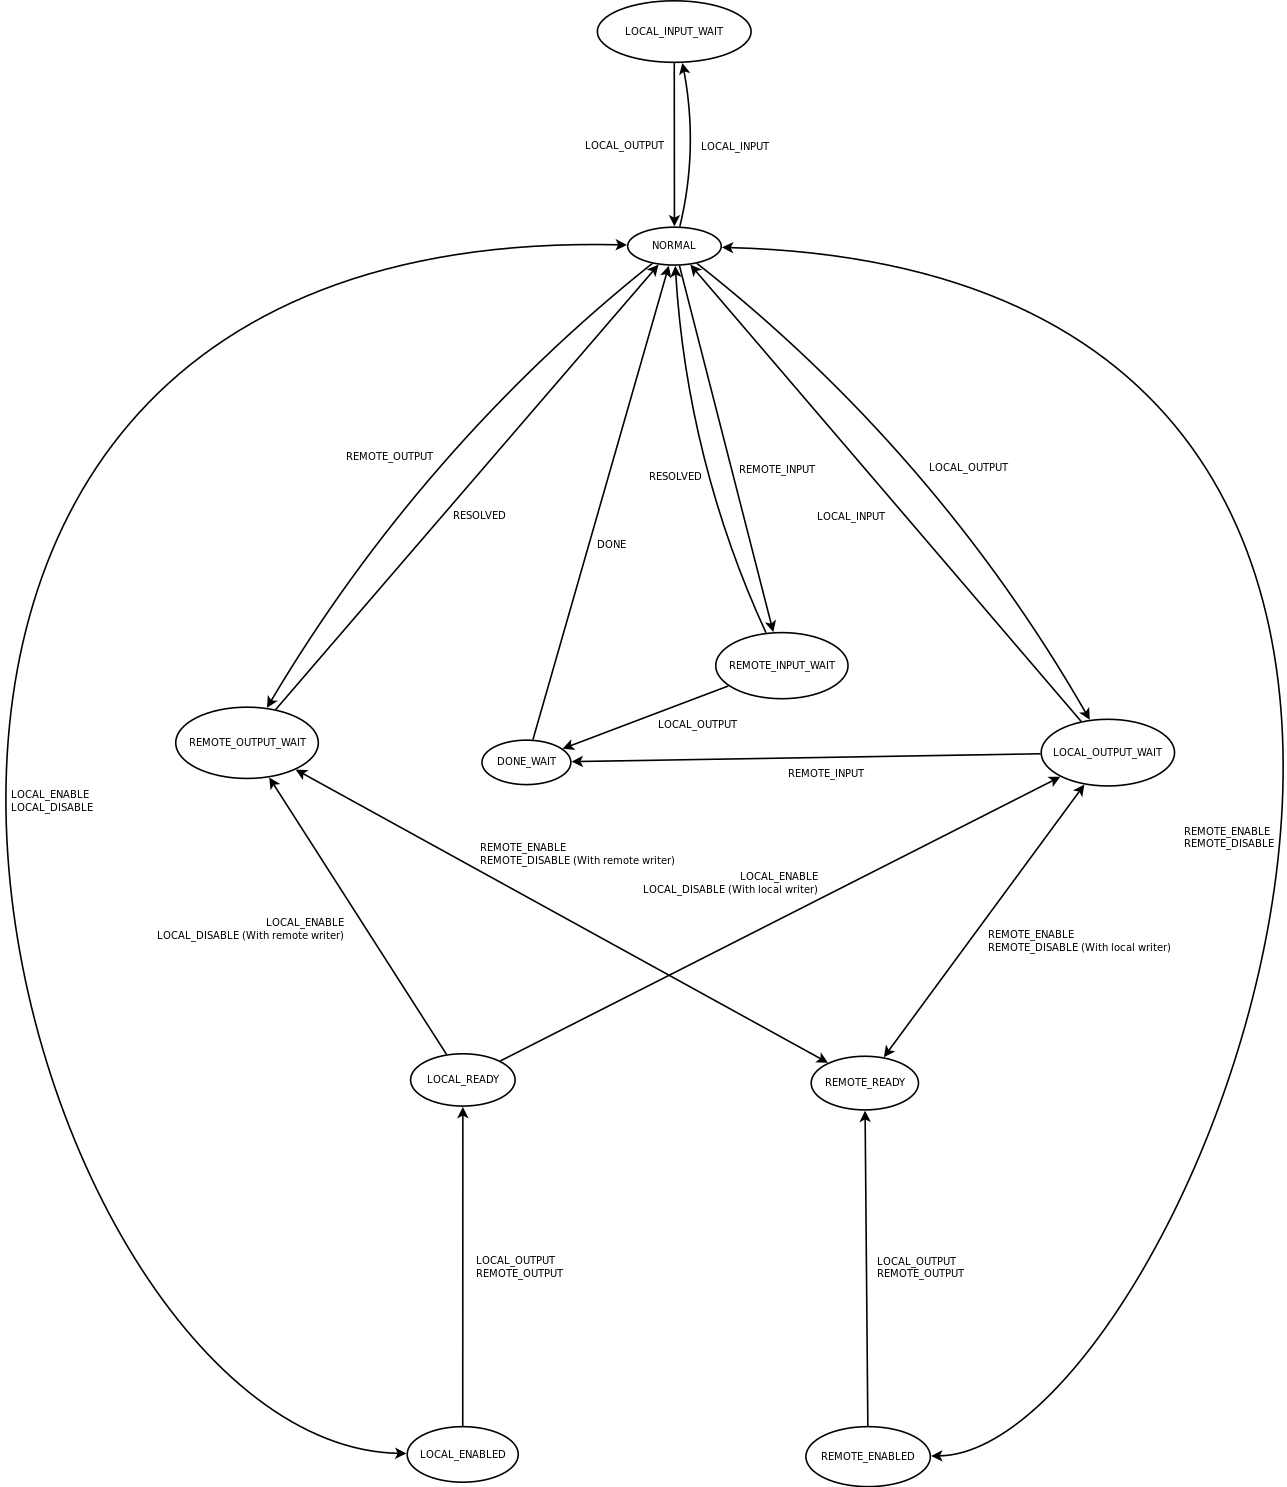
\includegraphics[width=\textwidth]{diagrams/channel_server}
  \caption{
    The state transition diagram for a channel, according to the channel
    server.
  }
  \label{channel-server}
\end{figure}

\subsection{Instance}

The \texttt{Instance} class is a subclass of the \texttt{VM} class, which adds
two new operations to allow remote instances to be created:
\begin{itemize}
  \item
    \texttt{STARTI} - Start Instance. This command takes an instruction pointer
    and a workspace size and instructs the process master to spawn a new
    instance with a workspace of the given size, which should execute the code
    pointed to by the instruction pointer. Furthermore, the third argument is
    the address of a word in the workspace of the local process. When the new
    instance is started, the value stored in this workspace location will be
    written to workspace location 0 of the new instance. This allows replication
    variables to be implemented more efficiently than if they had to be
    transferred by a channel. Once the value has been sent, the workspace
    address in the local machine is associated with the child instance, and must
    be joined upon before the parent can exit.
  \item
    \texttt{JOINI} - Join Instance. This takes a workspace address as an
    argument and waits for the associated instance to exit. If it has already
    exited then this instruction returns immediately.
\end{itemize}
These instructions are implemented so that if they block, a different process on
the same instance may continue to run in the meantime.

In addition to these new instructions, \texttt{Instance} reimplements the
channel instructions so that they delegate to the \texttt{ChannelServer}. This
comes at a performance cost when compared to the internal channels that the base
class uses, but allows true parallelism to be utilised.
